\documentclass[11pt]{article}

\usepackage[T1]{fontenc}
\usepackage[utf8]{inputenc}
\usepackage{lmodern}
\usepackage[margin=1in]{geometry}
\usepackage{amsmath}
\usepackage{amssymb}
\usepackage{amsthm}
\usepackage{mathtools}
\usepackage{graphicx}
\usepackage{xcolor}
\usepackage{listings}
\usepackage{microtype}
\usepackage{hyperref}
\Urlmuskip=0mu plus 1mu\relax

\definecolor{codebackground}{RGB}{247,247,247}
\definecolor{codecomment}{RGB}{72,112,72}
\definecolor{codekeyword}{RGB}{32,74,135}
\definecolor{codestring}{RGB}{164,0,0}

\lstdefinestyle{scala}{
  backgroundcolor=\color{codebackground},
  basicstyle=\ttfamily\small,
  breakatwhitespace=true,
  breaklines=true,
  columns=fixed,
  commentstyle=\color{codecomment},
  frame=single,
  keepspaces=true,
  keywordstyle=\color{codekeyword}\bfseries,
  language=Scala,
  numbers=none,
  showspaces=false,
  showstringspaces=false,
  showtabs=false,
  stringstyle=\color{codestring},
  tabsize=2
}

\hypersetup{
  colorlinks=true,
  linkcolor=blue,
  citecolor=blue,
  urlcolor=blue,
  pdftitle={Formal Verification of Cyclic Lists},
  pdfauthor={Thiago Henrique Mata}
}

\title{Formal Verification of Cyclic Lists}
\author{%
  Thiago Henrique Mata\\
  \small Independent Researcher\\
  \small \href{mailto:thiago.henrique.mata@gmail.com}{thiago.henrique.mata@gmail.com}\\
  \small \url{https://thiagomata.com/}\\
  \small \url{https://github.com/thiagomata}
}
\date{}

\begin{document}

\maketitle

\begin{abstract}
In previous articles, we defined bounded Lists and Integrals of
\texttt{BigInt} from scratch, relying only on core type constructs and
recursion, with no prior knowledge of Scala's collections required. From that,
we proved and formally verified some properties related to them as size,
append, concat, slice and sum. This article uses that as a foundation to define
Cycles --- unbounded List of Integers created from a bounded List, where the
values of the Cycle are the values of the List in repetition using recursion.
Then, we formally defined and verified key properties such as cycle equivalence
between definitions, element access via modular indexing, and periodic
invariance using the Stainless verification system. All properties are
expressed and proved within a minimal framework using only elementary
arithmetic, recursion, and pure Scala code. This work bridges mathematical
foundations and executable verification, offering a self-contained, verifiable
approach of modular arithmetic.
\end{abstract}


\begin{center}
  \small Licensed under the Creative Commons Attribution 4.0 International
  License (CC BY 4.0): \url{https://creativecommons.org/licenses/by/4.0/}.
\end{center}

\section{Introduction}

Unbounded lists in cycles, are a fundamental concept in computer science and
mathematics, often used to model repetitive structures or processes. They can
be thought of as infinite lists that repeat a finite sequence of elements.

\begin{equation*}
\begin{aligned}
L &= [x_0, x_1, x_2, \ldots, x_{n-1}]
  \mid x_n \in \mathbb{S}, L \in \mathbb{L} \\
\operatorname{Cycle}(L)
  &= [x_0, x_1, x_2, \ldots, x_{n-1}, x_0, x_1, \ldots]
\end{aligned}
\end{equation*}

In this article, we present discrete definition of Cycle operations over finite
integer lists, defined recursively and verified some of its properties using
the Stainless system. Our approach follows a zero-prior-knowledge philosophy,
building on a previously verified foundation for recursive list structure. The
result is a verified, from-scratch implementation of cycle operations, suitable
as a foundation for higher-level numeric reasoning over unbounded lists.

This article verifies:

\begin{itemize}
  \item Cycle definitions: recursive, modulo, and memory --- Section~3.
  \item Equivalence: recursive and modulo produce identical values at every
    position --- Section~4.
  \item Element access: modular indexing, small-position direct lookup ---
    Subsections~5.1--5.2.
  \item Periodic invariance: value unchanged by adding cycle-period multiples
    --- Subsections~5.3--5.4.
  \item Mod propagation: remainder computed from base-cycle values ---
    Subsection~5.5.
  \item Repeated-cycle invariance: repeating the base list preserves all
    lookups --- Subsection~5.6.
  \item Cycle value positivity: all values $\geq 0$ at every position ---
    Subsection~5.7.
  \item Cycle rotation: rotates base list, shifts index --- Subsection~5.8.
  \item Residue classification: all-zero, none-zero, and some-zero divisor
    classifications transfer from the base list to every cycle position ---
    Subsections~5.10--5.12.
\end{itemize}

\subsection{Related work}

Finite rotation already has a substantial formal treatment in Lean's Mathlib:
it includes rotation reduced modulo list length, indexed rotation laws, and an
equivalence relation identifying rotated lists~\cite{leanmathlibrotate}. These
results give a close formal point of contact for the article's base-list
rotation and modular-indexing laws.

There is also broader work on cyclic datatypes as recursive programming
structures. Hamana studies cyclic lists and related data modulo bisimulation,
with a semantic account of their computation rules~\cite{hamana2017cyclic}.
That setting is more general and different from the present periodic sequence
generated by a finite integer list. Together, these sources place the Stainless
development between finite-list rotation and general cyclic-data theory, while
this article verifies the equivalence of its recursive and modulo presentations
and the period, residue, and lookup properties of its concrete periodic model.


\section{Preliminaries}

We reuse several basic list operations and their verified properties from the
companion articles \href{https://github.com/thiagomata/prime-numbers/blob/cycle-article-v1.0.0/articles/chapter3/list.md}{\emph{Using Formal Verification to Prove Properties of Lists Recursively Defined}}~\cite{mata2026lists}
and \href{https://github.com/thiagomata/prime-numbers/blob/cycle-article-v1.0.0/articles/chapter4/integral.md}{\emph{Formal Verification of Discrete Integration Properties from First Principles}}~\cite{mata2026integral}.

These articles also defined and verified their properties using the same
zero-prior-knowledge methodology, and are treated here as foundational
primitives.

For any list $L$ of numeric values $x_i \in \mathbb{S}$ where $\mathbb{S}$ is
a set of all numeric values, $\mathbb{L}$ is the the set of all lists, and $n$
is the size of the list, we define:

\begin{equation*}
\begin{aligned}
L_e &\in \mathbb{L} \\
L_e &= []
\end{aligned}
\end{equation*}

\begin{equation*}
\begin{aligned}
&\text{head} \in \mathbb{S} \\
&\text{tail} \in \mathbb{L} \\
&L_{node}(\text{head}, \text{tail}) \in \mathbb{L}_{node}
\end{aligned}
\end{equation*}

\begin{equation*}
\mathbb{L} = \{L_e\} \cup
\{L_{node}(\text{head}, \text{tail})
\mid \text{head} \in \mathbb{S},\ \text{tail} \in \mathbb{L}\}
\end{equation*}

\begin{equation*}
L = [x_0, x_1, \dots, x_{n-1}] \in \mathbb{S}^n
\end{equation*}

\begin{equation*}
\begin{aligned}
\operatorname{size}(L) &:=
\begin{cases}
0 & \text{if } L = L_e \\
1 + \operatorname{size}(\operatorname{tail}(L)) & \text{otherwise}
\end{cases} \\
\operatorname{sum}(L) &:=
\begin{cases}
0 & \text{if } L = L_e \\
\operatorname{head}(L) + \operatorname{sum}(\operatorname{tail}(L))
  & \text{otherwise}
\end{cases}
\end{aligned}
\end{equation*}

\begin{equation*}
\begin{gathered}
\begin{aligned}
|L| > 0 \implies \operatorname{last}(L) &:=
\begin{cases}
\operatorname{head}(L) & \text{if } |L| = 1 \\
\operatorname{last}(\operatorname{tail}(L)) & \text{otherwise}
\end{cases} \\
|L| > 0 \implies \operatorname{slice}(L,f,t) &:=
\begin{cases}
[L_j] & \text{if } f = t \\
\operatorname{slice}(L,f,t-1) \mathbin{\texttt{++}} [L_t]
  & \text{if } f < t
\end{cases}
\end{aligned}
\\[0.5ex]
\forall\, f,t \in \mathbb{N}\ \text{where } 0 \leq f \leq t
\end{gathered}
\end{equation*}

\begin{equation*}
\begin{aligned}
A \mathbin{\texttt{++}} B &:=
\begin{cases}
B & \text{if } A = L_e \\
L_{node}(\operatorname{head}(A),
  \operatorname{tail}(A) \mathbin{\texttt{++}} B) & \text{otherwise}
\end{cases}
\end{aligned}
\end{equation*}

\begin{equation*}
\forall\, L,A,B \in \mathbb{L}
\end{equation*}

From these definitions, the authors~\cite{mata2026lists} mathematically prove
and formally verify the following properties of lists:

\begin{equation*}
\forall\, L,A,B \in \mathbb{L},\quad
\forall\, v \in \mathbb{S},\quad
\forall\, i,f,t \in \mathbb{N}
\end{equation*}

\begin{equation*}
f > t,\quad 0 \leq i < |L|
\end{equation*}

\begin{equation*}
\begin{aligned}
|L| > 0 &\implies \operatorname{tail}(L)
  = L[x_1,x_2,\dots,x_{n-1}] \quad \text{[Tail Identity]} \\
|L| > 0 &\implies L_0 = \operatorname{head}(L)
  \quad \text{[Head Identity]} \\
|L| > 0 &\implies L_{|L|-1} = \operatorname{last}(L)
  \quad \text{[Last Element Identity]} \\
|L|-1 > i > 0 &\implies L_i = \operatorname{tail}(L)_{i-1}
  \quad \text{[Access Tail Shift Left]} \\
|L|-2 > i > 1 &\implies \operatorname{tail}(L)_i = L_{i+1}
  \quad \text{[Access Tail Shift Right]}
\end{aligned}
\end{equation*}

\begin{equation*}
\begin{aligned}
|L| &= \operatorname{size}(L) \quad \text{[Size Identity]} \\
\sum L &= \operatorname{sum}(L) \quad \text{[Sum matches Summation]} \\
\sum (v :: L) &= v + \sum L \quad \text{[Left Append Preserves Sum]} \\
\sum (A \mathbin{\texttt{++}} B) &= \sum A + \sum B
  \quad \text{[Sum over Concatenation]} \\
\sum (A \mathbin{\texttt{++}} B) &=
  \sum (B \mathbin{\texttt{++}} A)
  \quad \text{[Commutativity of Sum over Concatenation]} \\
L[f \dots t] &= L[f \dots (t-1)] \mathbin{\texttt{++}} [L_t]
  \quad \text{[Slice Append Consistency]}
\end{aligned}
\end{equation*}


\section{Cycle Definitions}

Building on the definitions and properties of lists, we now define Cycles.

A Cycle is an unbounded list that repeats a finite sequence of elements from a
bounded list. In this study, we restrict our universe of values $\mathbb{S}$ to
be the set of non-negative integers, i.e., $\mathbb{S}=\mathbb{N}_0$.

\begin{itemize}
  \item Recursive: values at $i$ where $i<n$ come from the base list,
    otherwise recurse on $i-n$ --- the definitional spec.
  \item Modulo: values come directly from the base list at position
    $i\bmod n$ --- efficient access.
  \item Memory: wraps \texttt{ModCycle}, adds classification tracking via
    \texttt{checkMod(d)} --- remembers which divisors produce all-zero,
    some-zero, or none-zero residue patterns.
\end{itemize}

\begin{figure}[htbp]
  \centering
  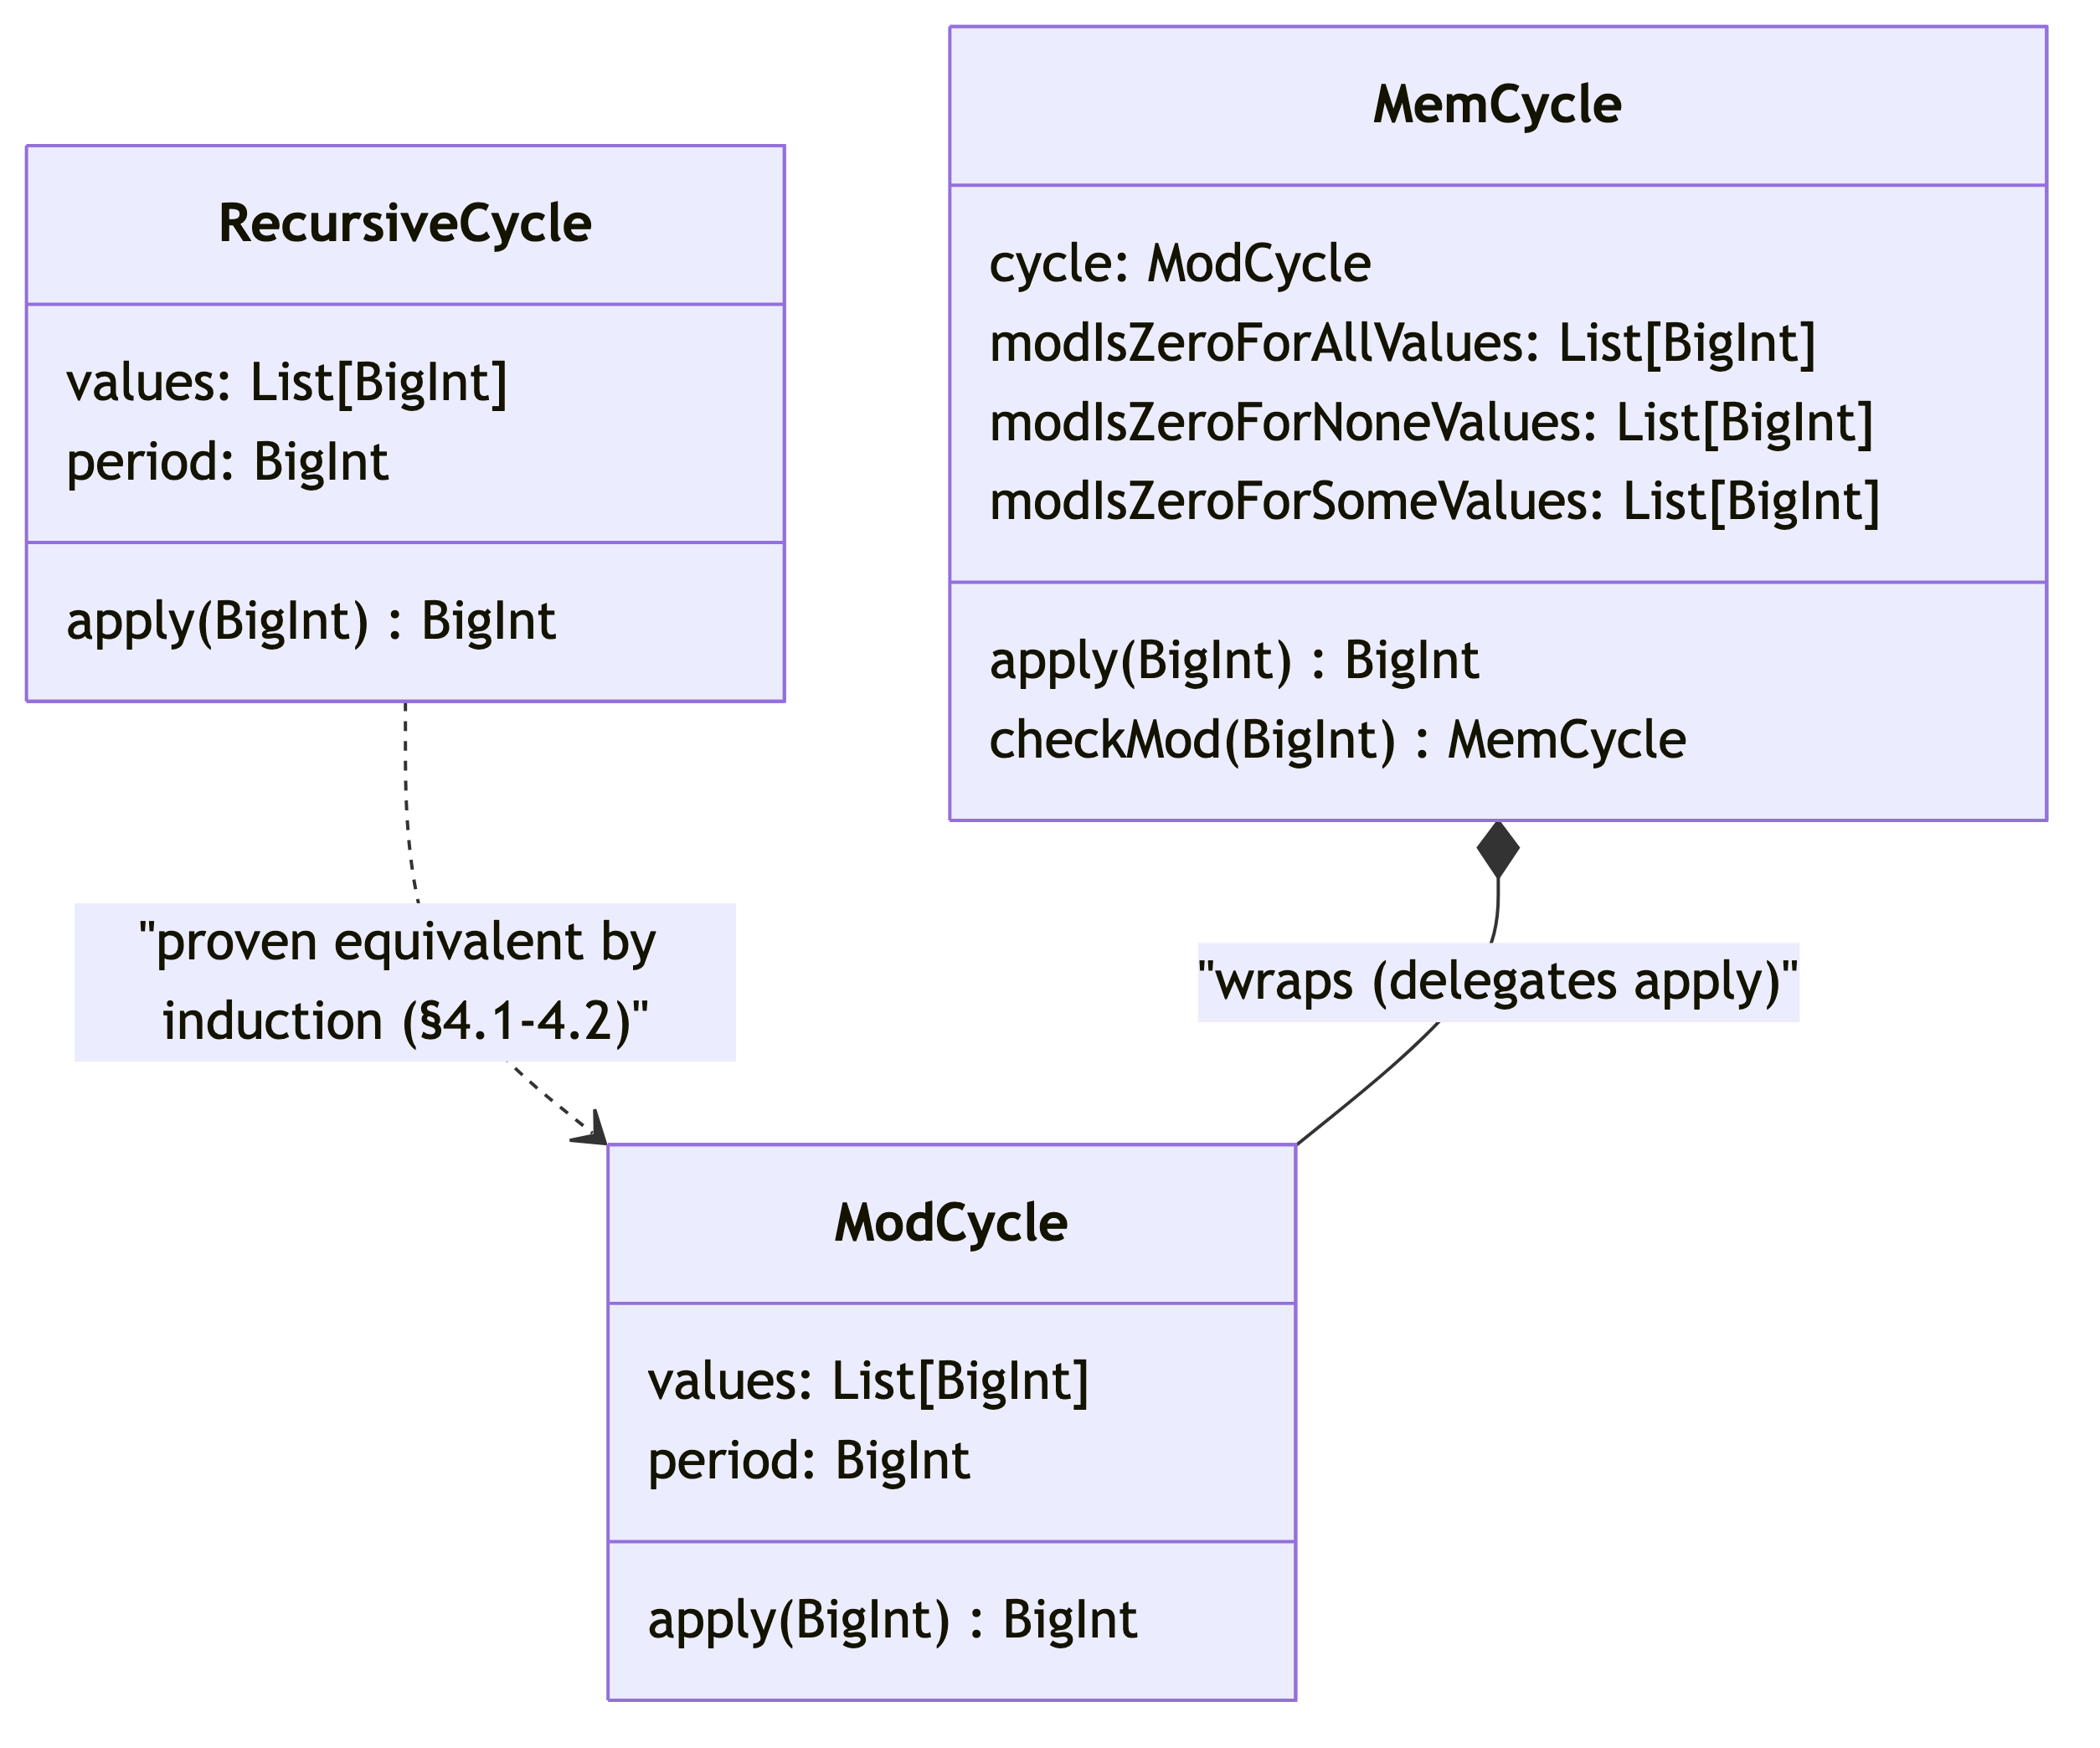
\includegraphics[width=0.92\linewidth]{figures/cycle-classes.png}
\end{figure}

\subsection{Recursive Cycle}

\begin{equation*}
\begin{aligned}
\forall\, L\in\mathbb{L},\quad \forall\, v&\in\mathbb{N}_0,
  \quad \forall\, i\in\mathbb{N}_0 \\
L &:= [v_0,v_1,\dots,v_{n-1}]\in\mathbb{N}_0^n \\
n &= |L| \\
\operatorname{RecCycle}_i &:=
\begin{cases}
L_i & \text{if } i<n \\
\operatorname{RecCycle}_{i-n} & \text{if } i\geq n
\end{cases},\quad |L|>0 \\
&\therefore \\
\operatorname{RecCycle}
  &= [v_0,v_1,\dots,v_{n-1},v_0,v_1,\dots] \\
\operatorname{Cycle}_i &:= \operatorname{RecCycle}_i
\end{aligned}
\end{equation*}

We take this recursive unrolling as the formal ground truth for the informal
picture of ``the infinite periodic sequence'' used throughout this article:
from here on, \texttt{Cycle} means \texttt{RecCycle}. That is a naming choice,
not a theorem --- the recursion peels off one copy of the base list per step,
which is exactly what the periodic sequence means. What still needs proof is
whether the modulo-based definition below computes the same values; that
equivalence is proved in Section~4.

The recursive cycle is defined at
\href{https://github.com/thiagomata/prime-numbers/blob/cycle-article-v1.0.0/src/main/scala/v1/chapter4/cycle/recursive/RecursiveCycle.scala}{\texttt{RecursiveCycle}}:

\begin{lstlisting}[style=scala]
case class RecursiveCycle(values: List[BigInt]) {
  require(values.nonEmpty)
  require(CycleUtils.checkPositiveOrZero(values))

  def period: BigInt = values.size

  def apply(position: BigInt): BigInt = {
    decreases(position)
    require(position >= 0)

    if (position < period) {
      values(position)
    } else {
      apply(position - values.size)
    }
  }
}
\end{lstlisting}

\subsection{Modulo Cycle}

A Cycle can also be defined using modulo arithmetic, which is a common approach
in computer science to handle cyclic structures.

\begin{equation*}
\begin{aligned}
\forall\, L\in\mathbb{L},\quad \forall\, v&\in\mathbb{N}_0,
  \quad \forall\, i\in\mathbb{N}_0 \\
L &:= [v_0,v_1,\dots,v_{n-1}]\in\mathbb{N}_0^n \\
n &= |L| \\
\operatorname{ModCycle}_i &= L[i\operatorname{mod}n],\quad |L|>0 \\
&\therefore \\
\operatorname{ModCycle}
  &= [v_0,v_1,\dots,v_{n-1},v_0,v_1,\dots]
\end{aligned}
\end{equation*}

This unrolls informally to the same picture, but nothing so far shows that
\texttt{ModCycle} and \texttt{RecCycle} --- which Subsection~3.1 took as the
meaning of \texttt{Cycle} --- agree at every index. One recurses by repeated
subtraction, the other computes a single remainder, and it is not obvious a
priori that the two produce the same sequence. Section~4 proves they do, which
is what lets \texttt{ModCycle} stand in for \texttt{Cycle} as well.

The modulo cycle is defined at
\href{https://github.com/thiagomata/prime-numbers/blob/cycle-article-v1.0.0/src/main/scala/v1/chapter4/cycle/mod/ModCycle.scala}{\texttt{ModCycle}}:

\begin{lstlisting}[style=scala]
case class ModCycle(values: List[BigInt]) {
  require(CycleUtils.checkPositiveOrZero(values))
  require(values.nonEmpty)

  def apply(position: BigInt): BigInt = {
    require(position >= 0)
    val index = Calc.mod(position, values.size)
    assert(index >= 0)
    assert(index < values.size)
    values(index)
  }

  def period: BigInt = values.size

  def sum(): BigInt = ListUtils.sum(values)
}
\end{lstlisting}

\subsection{Memory Cycle}

The third representation, \texttt{MemCycle}, wraps a \texttt{ModCycle} and
adds classification state: three lists tracking which divisors produce
all-zero, some-zero, or none-zero residue patterns across the cycle's values.

Like ModCycle, positional lookup uses modular indexing; value access delegates
directly to the wrapped ModCycle. Positional equivalence between the two is
immediate by construction: \texttt{MemCycle.apply(position)} calls the wrapped
\texttt{cycle(position)}, and \texttt{MemCycle(values)} constructs that wrapped
cycle as \texttt{ModCycle(values)}.

\begin{equation*}
\begin{aligned}
\operatorname{MemCycle}(L)_i
  &= \operatorname{ModCycle}(L)_i
  && \text{[By MemCycle.apply delegating to its wrapped ModCycle]}
\end{aligned}
\end{equation*}

The bounded bridge
\href{https://github.com/thiagomata/prime-numbers/blob/cycle-article-v1.0.0/src/main/scala/v1/chapter4/cycle/properties/CycleProperties.scala}{\texttt{CycleProperties::assertModCycleEqualsMemCycle}}
verifies the same lookup equality over one physical period for a
\texttt{ModCycle} and a \texttt{MemCycle} sharing the same values and period.

\texttt{MemCycle(L)} returns the same values as \texttt{ModCycle(L)} by
definition: it stores \texttt{ModCycle(L)} and delegates every lookup to it.
Section~4 proves the remaining piece --- that \texttt{RecursiveCycle(L)} and
\texttt{ModCycle(L)} also agree at every position --- after which the full
three-way equality chain used throughout the article is assembled at the close
of that section.

The cycle is immutable. Calling \texttt{checkMod(d)} returns a \emph{new}
\texttt{MemCycle} with \texttt{d} added to the appropriate classification
list. The original is unchanged. Values are never modified; classification is
metadata accumulated across calls.

\begin{lstlisting}[style=scala]
case class MemCycle private (
  cycle: ModCycle,
  modIsZeroForAllValues: List[BigInt] = List.empty,
  modIsZeroForNoneValues: List[BigInt] = List.empty,
  modIsZeroForSomeValues: List[BigInt] = List.empty,
) {
  def apply(position: BigInt): BigInt = cycle(position)
  def values: List[BigInt] = cycle.values
  def period: BigInt = cycle.period
  def checkMod(dividend: BigInt): MemCycle = { /* returns new MemCycle */ }
}
\end{lstlisting}

The memory cycle is defined at
\href{https://github.com/thiagomata/prime-numbers/blob/cycle-article-v1.0.0/src/main/scala/v1/chapter4/cycle/memory/MemCycle.scala}{\texttt{MemCycle}}.
Classification lemmas are verified in
\href{https://github.com/thiagomata/prime-numbers/blob/cycle-article-v1.0.0/src/main/scala/v1/chapter4/cycle/memory/properties/CycleCheckMod.scala}{\texttt{CycleCheckMod}}.


\section{Cycle Equivalence}

Subsection~3.1 defines \texttt{Cycle} to mean \texttt{RecCycle} --- a naming
choice, not a claim. This section proves the claim that actually needs proving:
that \texttt{ModCycle}, defined independently by a single modulo operation
rather than by recursive unrolling, computes exactly the same values as
\texttt{RecCycle} at every position. This equivalence is what the rest of the
article leans on whenever it moves between the two representations, and it is
not immediate from the two definitions side by side. We prove it by induction
on the position $i$.

\begin{itemize}
  \item Base case ($i<n$): both definitions consult the base list directly at
    the same position.
  \item Inductive step ($i\geq n$): the recursive definition reduces to $i-n$,
    wrapping to the same modulo position.
\end{itemize}

\begin{equation*}
\begin{aligned}
\forall\, L\in\mathbb{L},\quad \forall\, v&\in\mathbb{N}_0,
  \quad \forall\, i\in\mathbb{N}_0 \\
L &:= [v_0,v_1,\dots,v_{n-1}]\in\mathbb{N}_0^n \\
n &= |L| \\
\operatorname{ModCycle}_i &= L[i\operatorname{mod}n],\quad |L|>0 \\
\operatorname{RecCycle}_i &=
\begin{cases}
L_i & \text{if } i<n \\
\operatorname{RecCycle}_{i-n} & \text{if } i\geq n
\end{cases},\quad |L|>0
\end{aligned}
\end{equation*}

\subsection{Base Case (\texorpdfstring{$i<n$}{i < n})}

When the position is within the first cycle, both definitions return the list
element directly.

\begin{equation*}
\begin{aligned}
i<n \implies i\operatorname{mod}n &= i
  && \text{[Trivial Mod For Small Dividend]} \\
\operatorname{ModCycle}_i &= L_{(i\operatorname{mod}n)}
  && \text{[ModCycle Definition]} \\
&=L_i && \text{[Since }i<n\text{, }i\operatorname{mod}n=i\text{]} \\
\operatorname{RecCycle}_i &= L_i
  && \text{[Since }i<n\text{, by RecCycle Definition]} \\
&\therefore \\
i<n \implies \operatorname{ModCycle}_i &= \operatorname{RecCycle}_i
  \quad \blacksquare && \text{[Q.E.D.]}
\end{aligned}
\end{equation*}

The lemma
\href{https://github.com/thiagomata/prime-numbers/blob/cycle-article-v1.0.0/articles/chapter2/modulo.md#61-trivial-case}{Trivial Mod for Small Dividend}
was proved and verified in the article
\href{https://github.com/thiagomata/prime-numbers/blob/cycle-article-v1.0.0/articles/chapter2/modulo.md}{\emph{Division and Modulo from Recursive Normalization}}~\cite{mata2026modulo}.

{\raggedright
This property is verified in
\href{https://github.com/thiagomata/prime-numbers/blob/cycle-article-v1.0.0/src/main/scala/v1/chapter4/cycle/recursive/properties/RecursiveCycleMatchesModCycle.scala}{\texttt{RecursiveCycleMatchesModCycle::}\allowbreak\texttt{assertCycleAndRecursiveCycleMathForSmallValues}}.
The full Scala verification code is in Appendix~A.1.
\par}

\subsection{Inductive Step (\texorpdfstring{$i\geq n$}{i >= n})}

For positions beyond the first cycle, both definitions reduce the position by
the cycle period and rely on the inductive hypothesis.

\begin{equation*}
\begin{aligned}
\operatorname{ModCycle}_{(i-n)} &= \operatorname{RecCycle}_{(i-n)}
  && \text{[By Induction Hypothesis]} \\
i\geq n \implies i\operatorname{mod}n
  &= (i-n)\operatorname{mod}n
  && \text{[Quotient Invariance Under Linear Shift]} \\
\operatorname{ModCycle}_i &= L_{(i\operatorname{mod}n)}
  && \text{[ModCycle Definition]} \\
&=L_{((i-n)\operatorname{mod}n)}
  && \substack{\text{[Since }i\geq n\text{, }i\operatorname{mod}n
       =(i-n)\operatorname{mod}n\text{]}} \\
&=\operatorname{ModCycle}_{(i-n)} && \text{[By Definition]} \\
&=\operatorname{RecCycle}_{(i-n)} && \text{[By Substitution]} \\
\operatorname{RecCycle}_i &= \operatorname{RecCycle}_{(i-n)}
  && \text{[By RecCycle Definition]} \\
&=\operatorname{ModCycle}_i && \text{[By Substitution]} \\
&\therefore \\
i\geq n \implies \operatorname{ModCycle}_i &= \operatorname{RecCycle}_i
  \quad \blacksquare && \text{[Q.E.D.]}
\end{aligned}
\end{equation*}

The lemma
\href{https://github.com/thiagomata/prime-numbers/blob/cycle-article-v1.0.0/articles/chapter2/modulo.md#65-quotient-invariance-under-linear-shift}{Quotient Invariance Under Linear Shift}
was proved and verified in
\href{https://github.com/thiagomata/prime-numbers/blob/cycle-article-v1.0.0/articles/chapter2/modulo.md}{\emph{Division and Modulo from Recursive Normalization}}~\cite{mata2026modulo}.

{\raggedright
This property is verified in
\href{https://github.com/thiagomata/prime-numbers/blob/cycle-article-v1.0.0/src/main/scala/v1/chapter4/cycle/recursive/properties/RecursiveCycleMatchesModCycle.scala}{\texttt{RecursiveCycleMatchesModCycle::}\allowbreak\texttt{assertCycleAndRecursiveCycleMathForAnyValues}}.
The full Scala verification code is in Appendix~A.2.
\par}

With both pieces now established --- \texttt{RecCycle} and \texttt{ModCycle}
equal by this section, \texttt{MemCycle} and \texttt{ModCycle} equal by
delegation (Subsection~3.3) --- the three representations agree at every
position:

\begin{equation*}
\begin{aligned}
\operatorname{RecCycle}(L)_i
  &=\operatorname{ModCycle}(L)_i && \text{[Subsections 4.1--4.2]} \\
  &=\operatorname{MemCycle}(L)_i && \text{[Subsection 3.3]} \\
\therefore\quad \operatorname{RecCycle}(L)_i
  &=\operatorname{ModCycle}(L)_i=\operatorname{MemCycle}(L)_i
  && \text{[Three-Way Equality]}
\end{aligned}
\end{equation*}


\section{Cycle Properties}

In this section, we prove and verify the main properties of Cycles. Each
property is stated mathematically, then shown to hold via a corresponding
verified lemma in Scala using the Stainless system.

\begin{itemize}
  \item Element access: \texttt{cycle(key) == cycle.values(mod(key, period))}
    --- Subsection~5.1.
  \item Small-value direct lookup: \texttt{key < period} $\Rightarrow$
    \texttt{cycle(key) == cycle.values(key)} --- Subsection~5.2.
  \item Periodicity:
    $\operatorname{cycle}(\text{key})=
    \operatorname{cycle}(\text{key}+\text{period}\cdot m)$ for any number of
    loops --- Subsection~5.3.
  \item Multi-loop consistency: value at \texttt{key} is independent of which
    multiple of the period is added --- Subsection~5.4.
  \item Mod propagation: remainder modulo $d$ at any position equals remainder
    at the base position --- Subsection~5.5.
  \item Repeated-cycle invariance: repeating the base list preserves all
    lookups --- Subsection~5.6.
  \item Value positivity: non-negative base values guarantee non-negative cycle
    values --- Subsection~5.7.
  \item Rotation: rotating the base list shifts the cycle index by the same
    amount --- Subsection~5.8.
  \item MemCycle-level restatements: the key access and modulo properties are
    also verified directly for the memory-backed representation ---
    Subsection~5.9.
  \item Residue classification transfer: all-zero, none-zero, and some-zero
    divisor classifications on the base list hold at every cycle position ---
    Subsections~5.10--5.12.
\end{itemize}

Throughout this section, $L$ is the finite backing list, $n$ is the period,
and $Cycle$ is the unbounded periodic stream it defines --- formally,
\texttt{Cycle} means \texttt{RecCycle} (Subsection~3.1), proved in Section~4 to
equal \texttt{ModCycle} at every position:

\begin{equation*}
\begin{aligned}
\forall\,L\in\mathbb{L},\quad \forall\,v&\in\mathbb{N}_0,
  \quad \forall\,i\in\mathbb{N}_0 \\
L &:= [v_0,v_1,\dots,v_{n-1}]\in\mathbb{N}_0^n,\quad |L|>0 \\
\operatorname{Cycle} &:= [v_0,v_1,\dots,v_{n-1},v_0,v_1,\dots] \\
n &:= |L|
\end{aligned}
\end{equation*}

\subsection{Cycle Element Access}

The value of any element in a cycle equals the value of the underlying list at
the position modulo the cycle period.

\begin{equation*}
\operatorname{Cycle}_i=L[i\operatorname{mod}n]
\end{equation*}

\noindent\textbf{Proof.}

\begin{equation*}
\begin{aligned}
\operatorname{Cycle}_i &= \operatorname{RecCycle}_i
  && \text{[Subsection 3.1 Definition]} \\
&=\operatorname{ModCycle}_i && \text{[Section 4 Cycle Equivalence]} \\
&=L[i\operatorname{mod}n] && \text{[ModCycle Definition]}
\end{aligned}
\end{equation*}

\begin{equation*}
\therefore\quad \operatorname{Cycle}_i=L[i\operatorname{mod}n]
  \quad \blacksquare\ \text{[Q.E.D.]}
\end{equation*}

The Cycle Equivalence property was proved and verified in Section~4.

This property is verified in
\href{https://github.com/thiagomata/prime-numbers/blob/cycle-article-v1.0.0/src/main/scala/v1/chapter4/cycle/properties/CycleProperties.scala}{\texttt{CycleProperties::findValueInCycle}}.
The full Scala verification code is in Appendix~A.3.

\subsection{Small Value in Cycle}

For positions smaller than the cycle period, the cycle value equals the list
value at that position directly.

\begin{equation*}
i<n\implies\operatorname{Cycle}_i=L_i
\end{equation*}

\noindent\textbf{Proof.}

\begin{equation*}
\begin{aligned}
\operatorname{Cycle}_i &= \operatorname{RecCycle}_i
  && \text{[Subsection 3.1 Definition]} \\
i<n\implies\operatorname{RecCycle}_i &= L_i
  && \text{[RecCycle Definition]}
\end{aligned}
\end{equation*}

\begin{equation*}
\therefore\quad i<n\implies\operatorname{Cycle}_i=L_i
  \quad \blacksquare\ \text{[Q.E.D.]}
\end{equation*}

This step only needs the \texttt{Cycle := RecCycle} naming from
Subsection~3.1; the \texttt{ModCycle} side of the equivalence proved in
Section~4 is not required here.

This property is verified in
\href{https://github.com/thiagomata/prime-numbers/blob/cycle-article-v1.0.0/src/main/scala/v1/chapter4/cycle/properties/CycleProperties.scala}{\texttt{CycleProperties::smallValueInCycle}}.
The full Scala verification code is in Appendix~A.4.

\subsection{Value Match After Many Loops}

Cycle values remain invariant when adding any multiple of the cycle period to
the access key.

\begin{equation*}
\operatorname{Cycle}_{(i+n\cdot m)}=L[i\operatorname{mod}n]
\end{equation*}

\noindent\textbf{Proof.}

\begin{equation*}
\begin{aligned}
\operatorname{Cycle}_{(i+n\cdot m)}
  &=\operatorname{RecCycle}_{(i+n\cdot m)}
  && \text{[Subsection 3.1 Definition]} \\
  &=\operatorname{ModCycle}_{(i+n\cdot m)}
  && \text{[Section 4 Cycle Equivalence]} \\
  &=L[(i+n\cdot m)\operatorname{mod}n]
  && \text{[ModCycle Definition]} \\
  &=L[i\operatorname{mod}n]
  && \text{[Quotient Invariance Under Linear Shift by Multiplier]}
\end{aligned}
\end{equation*}

\begin{equation*}
\therefore\quad \operatorname{Cycle}_{(i+n\cdot m)}=L[i\operatorname{mod}n]
  \quad \blacksquare\ \text{[Q.E.D.]}
\end{equation*}

The lemma
\href{https://github.com/thiagomata/prime-numbers/blob/cycle-article-v1.0.0/articles/chapter2/modulo.md#65-quotient-invariance-under-linear-shift}{Quotient Invariance Under Linear Shift}
and its multiplier variant were proved and verified in
\emph{Division and Modulo from Recursive Normalization}~\cite{mata2026modulo}.

This property is verified in
\href{https://github.com/thiagomata/prime-numbers/blob/cycle-article-v1.0.0/src/main/scala/v1/chapter4/cycle/properties/CycleProperties.scala}{\texttt{CycleProperties::valueMatchAfterManyLoops}}.
The full Scala verification code is in Appendix~A.5.

\subsection{Two Multiples of Cycle Size}

Shifting the same key by two different multiples of the cycle period produces
the same cycle value either way.

\begin{equation*}
\operatorname{Cycle}_{(i+n\cdot m_1)}
  =\operatorname{Cycle}_{(i+n\cdot m_2)}
\end{equation*}

\noindent\textbf{Proof.} By Subsection~5.3, applied at both $m_1$ and $m_2$:

\begin{equation*}
\begin{aligned}
\operatorname{Cycle}_{(i+n\cdot m_1)}
  &=L[i\operatorname{mod}n]
  && \text{[Subsection 5.3, Value Match After Many Loops]} \\
\operatorname{Cycle}_{(i+n\cdot m_2)}
  &=L[i\operatorname{mod}n]
  && \text{[Subsection 5.3, Value Match After Many Loops]}
\end{aligned}
\end{equation*}

\begin{equation*}
\therefore\quad
\operatorname{Cycle}_{(i+n\cdot m_1)}
  =\operatorname{Cycle}_{(i+n\cdot m_2)}
  =L[i\operatorname{mod}n]
  \quad \blacksquare\ \text{[Q.E.D.]}
\end{equation*}

This property is verified in
\href{https://github.com/thiagomata/prime-numbers/blob/cycle-article-v1.0.0/src/main/scala/v1/chapter4/cycle/properties/CycleProperties.scala}{\texttt{CycleProperties::valueMatchAfterManyLoopsInBoth}}.
The full Scala verification code is in Appendix~A.6.

\subsection{Propagate Modulo from Value to Cycle}

The modulo operation applied to a cycle value can be equivalently applied to
the underlying list value at the modular index. Since the previous sections
prove that the cycle representations agree at every position, we can use the
modulo cycle definition directly: cycle lookup first reduces the position to
\texttt{i mod n}, and taking a remainder by any positive divisor \texttt{d}
preserves that same base-position reduction.

\begin{equation*}
\operatorname{Cycle}_i\operatorname{mod}d
  =L_{i\operatorname{mod}n}\operatorname{mod}d
\end{equation*}

\noindent\textbf{Proof.}

\begin{equation*}
\begin{aligned}
\operatorname{Cycle}_i
  &=\operatorname{RecCycle}_i && \text{[Subsection 3.1 Definition]} \\
  &=\operatorname{ModCycle}_i && \text{[Section 4 Cycle Equivalence]} \\
  &=L_{i\operatorname{mod}n} && \text{[ModCycle Definition]}
\end{aligned}
\end{equation*}

\begin{equation*}
\therefore\quad
\operatorname{Cycle}_i\operatorname{mod}d
  =L_{i\operatorname{mod}n}\operatorname{mod}d
  \quad \blacksquare\ \text{[Q.E.D.]}
\end{equation*}

This property is verified in
\href{https://github.com/thiagomata/prime-numbers/blob/cycle-article-v1.0.0/src/main/scala/v1/chapter4/cycle/properties/CycleProperties.scala}{\texttt{CycleProperties::propagateModFromValueToCycle}}.
The related idempotence restatement,
\texttt{cycle(position) == cycle(position mod period)}, is verified in
\href{https://github.com/thiagomata/prime-numbers/blob/cycle-article-v1.0.0/src/main/scala/v1/chapter4/cycle/properties/CycleProperties.scala}{\texttt{CycleProperties::assertCycleOfPosEqualsCycleOfModPos}}.
The full Scala verification code is in Appendix~A.7.

\subsection{Repeated-Cycle Invariance}

When a cycle's base list is repeated $t$ times to form a longer physical
period, the values read at every position remain identical. The repeated cycle
is structurally a concatenation of $t$ copies of the original list; the extra
length is invisible at any index because modular indexing composes correctly
across the nested periods. Repetition uses the same $t$-fold notation as
\href{https://github.com/thiagomata/prime-numbers/blob/cycle-article-v1.0.0/articles/chapter4/integral-cycle.md#61-integral-invariance-under-cycle-repetition}{\emph{Integral Cycle}, Subsection 6.1's $L^{(x)}$}
(list repeated $x$ times), defined the same way by unfolding one copy at a
time:

\begin{equation*}
\begin{aligned}
V^{(t)} &:={}
\begin{cases}
L_e & \text{if }t=0, \\
V\mathbin{\texttt{++}}V^{(t-1)} & \text{otherwise}.
\end{cases}
\end{aligned}
\end{equation*}

\begin{equation*}
\begin{aligned}
C &\text{ --- original MemCycle},\quad V=\operatorname{values}(C),
  \quad n=|V| \\
C^{(t)} &\text{ --- repeated cycle},\quad
  \operatorname{values}(C^{(t)})=V^{(t)}\quad\text{with }t>0 \\
\operatorname{period} &=t\cdot n
\end{aligned}
\end{equation*}

\noindent\textbf{Proof.}

\begin{equation*}
\begin{aligned}
C^{(t)}(\text{pos})
  &=V^{(t)}(\operatorname{mod}(\text{pos},\operatorname{period}))
  && \text{[MemCycle access via modular index]} \\
  &=V(\operatorname{mod}(\operatorname{mod}(\text{pos},t\cdot n),n))
  && \text{[Repeated list access pattern]} \\
  &=V(\operatorname{mod}(\text{pos},n))
  && \text{[ModOperations::modByPositiveMultipleThenBase]} \\
  &=C(\text{pos})
  && \text{[Original cycle access]} \\
  &\quad\blacksquare && \text{[Q.E.D.]}
\end{aligned}
\end{equation*}

The proof separates construction from lookup. Callers must build a valid
\texttt{MemCycle} from the repeated values; this lemma only says that once such
a cycle exists, the larger physical period does not change any lookup.

\begin{lstlisting}[style=scala]
def assertRepeatedValuesCycleMatches(
  cycle: MemCycle,
  repeatedCycle: MemCycle,
  times: BigInt,
  position: BigInt
): Boolean = {
  require(times > BigInt(0))
  require(position >= BigInt(0))
  require(cycle.period > BigInt(0))
  require(repeatedCycle.values == ListRepeatProperties.repeat(cycle.values, times))
  // ... inductive proof via mod composition ...
  repeatedCycle(position) == cycle(position)
}.holds
\end{lstlisting}

This property is verified in
\href{https://github.com/thiagomata/prime-numbers/blob/cycle-article-v1.0.0/src/main/scala/v1/chapter4/cycle/memory/properties/MemCycleProperties.scala}{\texttt{MemCycleProperties::assertRepeatedValuesCycleMatches}}.
The complete Scala derivation is included in Appendix~A.8.

\subsection{Cycle Value Positivity}

When every value in the base list is non-negative, every position in the cycle
returns a non-negative value. This guarantees that cycle lookups never produce
negative numbers, which is essential for integral and gap reasoning.

\begin{equation*}
\begin{aligned}
(\forall x\in L,\ x\geq 0)\land |L|>0
  \implies \operatorname{Cycle}_{\text{pos}}\geq 0
\end{aligned}
\end{equation*}

\noindent\textbf{Proof.} By Subsection~5.1,
$\operatorname{Cycle}_{\text{pos}}=L[\text{pos}\operatorname{mod}n]$, and
$\text{pos}\operatorname{mod}n$ is a valid index into $L$ (in $[0,n)$). So
$\operatorname{Cycle}_{\text{pos}}$ is one of the values of $L$---and every
value of $L$ is non-negative by hypothesis, so
$\operatorname{Cycle}_{\text{pos}}\geq 0$.

\begin{equation*}
\therefore\quad
(\forall x\in L,\ x\geq 0)\land |L|>0
  \implies \operatorname{Cycle}_{\text{pos}}\geq 0
  \quad \blacksquare\ \text{[Q.E.D.]}
\end{equation*}

This property is verified in
\href{https://github.com/thiagomata/prime-numbers/blob/cycle-article-v1.0.0/src/main/scala/v1/chapter4/cycle/properties/CycleProperties.scala}{\texttt{CycleProperties::cycleValuePositiveOrZero}},
which reduces to the list-level helper
\texttt{CycleUtils::checkPositiveOrZeroAtIndex}---indexing into a non-negative
list at a valid position yields a non-negative value. The full Scala
verification code is in Appendix~A.9.

The same argument gives the verified strict lower-bound form: if every base
value is greater than $x$, then every cycle value is greater than $x$.

\begin{equation*}
\begin{aligned}
(\forall y\in L,\ y>x)\land |L|>0
  &\implies \operatorname{Cycle}_{\text{pos}}>x.
\end{aligned}
\end{equation*}

\noindent\textbf{Proof.} The modular index selects a value of $L$, which is
greater than $x$ by hypothesis:

\begin{equation*}
\begin{aligned}
\operatorname{Cycle}_{\text{pos}}
  &=L[\text{pos}\operatorname{mod}n] && \text{[Subsection 5.1]} \\
L[\text{pos}\operatorname{mod}n]
  &>x && \text{[Base-list lower bound]} \\
\therefore\quad \operatorname{Cycle}_{\text{pos}}
  &>x.\quad \blacksquare\ \text{[Q.E.D.]}
\end{aligned}
\end{equation*}

{\raggedright
This strengthening is verified for \texttt{RecursiveCycle}, the article's
\texttt{Cycle} representation, in
\href{https://github.com/thiagomata/prime-numbers/blob/cycle-article-v1.0.0/src/main/scala/v1/chapter4/cycle/recursive/RecursiveCycle.scala#cycleValueBiggerThan}{\texttt{RecursiveCycle::cycleValueBiggerThan}}.
\par}

\subsection{Cycle Rotation}

Rotating a cycle's base list by $k$ positions and then accessing index $i$
gives the same value as accessing the original cycle at index $i+k$. This
connects cycle structure directly to the list rotation concept from chapter 3.
Rotation is defined by re-indexing the base list from offset $k$:

\begin{equation*}
\begin{aligned}
\operatorname{rotateAt}(L,k)
  &:=\big[\,L[(k+j)\operatorname{mod}n]\mid 0\leq j<n\,\big] \\
\operatorname{rotateAt}(\operatorname{Cycle},k)_i
  &:=\operatorname{rotateAt}(L,k)[i\operatorname{mod}n]
\end{aligned}
\end{equation*}

\begin{equation*}
\begin{aligned}
\operatorname{rotateAt}(\operatorname{Cycle},k)_i
  =\operatorname{Cycle}_{i+k}\quad\text{for }k\geq 0,\ i\geq 0
\end{aligned}
\end{equation*}

\noindent\textbf{Proof.}

\begin{equation*}
\begin{aligned}
\operatorname{rotateAt}(\operatorname{Cycle},k)_i
  &=\operatorname{rotateAt}(L,k)[i\operatorname{mod}n]
  && \text{[By Definition]} \\
  &=L[(k+(i\operatorname{mod}n))\operatorname{mod}n]
  && \substack{\text{[By Definition, since }i\operatorname{mod}n\\
                \text{ lies in }[0,n)\text{]}} \\
  &=L[(k+i)\operatorname{mod}n]
  && \substack{\text{[Modulo Idempotence + Distributivity}\\
                \text{over Addition]}} \\
  &=\operatorname{Cycle}_{i+k}
  && \text{[Subsection 5.1 Cycle Element Access]}
\end{aligned}
\end{equation*}

\begin{equation*}
\therefore\quad
\operatorname{rotateAt}(\operatorname{Cycle},k)_i
  =\operatorname{Cycle}_{i+k}\quad\text{for }k\geq 0,\ i\geq 0
  \quad \blacksquare\ \text{[Q.E.D.]}
\end{equation*}

The third step composes
\href{https://github.com/thiagomata/prime-numbers/blob/cycle-article-v1.0.0/articles/chapter2/modulo.md#68-modulo-idempotence}{Modulo Idempotence}
and
\href{https://github.com/thiagomata/prime-numbers/blob/cycle-article-v1.0.0/articles/chapter2/modulo.md#69-distributivity-over-addition}{Distributivity over Addition},
both proved and verified in
\emph{Division and Modulo from Recursive Normalization}~\cite{mata2026modulo}:
$\operatorname{mod}(k+\operatorname{mod}(i,n),n)
=\operatorname{mod}(k+i,n)$ follows because both sides reduce to
$\operatorname{mod}(\operatorname{mod}(k,n)+
\operatorname{mod}(i,n),n)$.

This property is verified in
\href{https://github.com/thiagomata/prime-numbers/blob/cycle-article-v1.0.0/src/main/scala/v1/chapter4/cycle/properties/CycleProperties.scala}{\texttt{CycleProperties::rotateAtValue}}.
The full Scala verification code is in Appendix~A.10.

\subsection{MemCycle-Level Restatement}

Sections~5.1--5.5 state element access, small-value lookup, periodic
invariance, multi-loop consistency, and mod propagation for \texttt{ModCycle}.
Since $\operatorname{MemCycle}(L)_i=\operatorname{ModCycle}(L)_i$ at every
position (Subsection~3.3, assembled at the close of Section~4), all five
results carry over to \texttt{MemCycle} by direct substitution---mathematically,
this section adds no content beyond Subsections~5.1--5.5. \texttt{MemCycle} is
nonetheless the representation actually used elsewhere in the codebase (it is
the one that carries residue-classification metadata), and Stainless has no way
to transfer a lemma proved for one concrete type to a different wrapper type
that merely happens to agree with it pointwise: each result below is re-proved
against \texttt{MemCycle}, and its proof body mirrors the corresponding
\texttt{ModCycle} lemma line for line rather than deriving anything new:

\begin{equation*}
\begin{aligned}
\operatorname{Cycle}_{\text{key}}
  &=L[\text{key}\operatorname{mod}n] && \text{[Element Access]} \\
\text{key}<n
  &\implies \operatorname{Cycle}_{\text{key}}=L[\text{key}]
  && \text{[Small Value Lookup]} \\
\operatorname{Cycle}_{\text{key}}
  &=\operatorname{Cycle}_{\text{key}+n\cdot m}
  && \text{[Periodic Invariance]} \\
\operatorname{Cycle}_{\text{key}+n\cdot m_1}
  &=\operatorname{Cycle}_{\text{key}+n\cdot m_2}
  && \text{[Multi-Loop Consistency]} \\
\operatorname{Cycle}_{\text{key}}\operatorname{mod}d
  &=L[\text{key}\operatorname{mod}n]\operatorname{mod}d
  && \text{[Mod Propagation]}
\end{aligned}
\end{equation*}

{\raggedright
These are verified in
\href{https://github.com/thiagomata/prime-numbers/blob/cycle-article-v1.0.0/src/main/scala/v1/chapter4/cycle/memory/properties/MemCycleProperties.scala}{\texttt{MemCycleProperties::findValueInCycle}},
\href{https://github.com/thiagomata/prime-numbers/blob/cycle-article-v1.0.0/src/main/scala/v1/chapter4/cycle/memory/properties/MemCycleProperties.scala}{\texttt{MemCycleProperties::smallValueInCycle}},
\href{https://github.com/thiagomata/prime-numbers/blob/cycle-article-v1.0.0/src/main/scala/v1/chapter4/cycle/memory/properties/MemCycleProperties.scala}{\texttt{MemCycleProperties::valueMatchAfterManyLoops}},
\href{https://github.com/thiagomata/prime-numbers/blob/cycle-article-v1.0.0/src/main/scala/v1/chapter4/cycle/memory/properties/MemCycleProperties.scala}{\texttt{MemCycleProperties::valueMatchAfterManyLoopsInBoth}},
and
\href{https://github.com/thiagomata/prime-numbers/blob/cycle-article-v1.0.0/src/main/scala/v1/chapter4/cycle/memory/properties/MemCycleProperties.scala}{\texttt{MemCycleProperties::propagateModFromValueToCycle}}.

The mod-idempotence identity from Subsection~5.5's proof (that
$\operatorname{Cycle}_i$ equals
$\operatorname{Cycle}_{(i\operatorname{mod}n)\operatorname{mod}n}$) has its
own \texttt{MemCycle} restatement in
\href{https://github.com/thiagomata/prime-numbers/blob/cycle-article-v1.0.0/src/main/scala/v1/chapter4/cycle/memory/properties/MemCycleProperties.scala}{\texttt{MemCycleProperties::assertCycleOfPosEqualsCycleOfModPos}}.
\par}

{\raggedright
\texttt{MemCycle} also classifies each divisor by how its residues behave
across the base list. \texttt{MemCycle.checkMod(d)} (Subsection~3.3) counts how
many values of $L$ are $\equiv 0\operatorname{mod}d$, via
\texttt{countModZero}---one pass over the list, adding 1 wherever the value is
$\equiv 0\operatorname{mod}d$:
\par}

\begin{equation*}
\begin{aligned}
\operatorname{countModZero}(L,d)&:={}
\begin{cases}
0 & \text{if }L=L_e, \\
1+\operatorname{countModZero}(\operatorname{tail}(L),d)
  & \text{if }\operatorname{head}(L)\operatorname{mod}d=0, \\
\operatorname{countModZero}(\operatorname{tail}(L),d)
  & \text{otherwise}.
\end{cases}
\end{aligned}
\end{equation*}

\texttt{checkMod(d)} then buckets $d$ as all-zero, none-zero, or some-zero
based on that count---each bucket defined and proved below to transfer from the
base list to every position of the infinite \texttt{Cycle}, using the same
move as Subsection~5.7: a cycle value is always \emph{some} value of $L$
(Subsection~5.1), so any property that holds of every value of $L$ holds of
every cycle position too. \texttt{CycleCheckMod.scala}'s ten lemmas separately
verify that the classification itself is mutually exclusive, exhaustive, and
persists correctly across independent \texttt{checkMod} calls---bookkeeping
properties of the classification lists, not further claims about cycle values,
so they are not restated here.

\subsection{All-Zero Residue Transfers to the Cycle}

\texttt{checkMod(d)} classifies \texttt{d} as all-zero when every value of
\texttt{L} is $\equiv 0\operatorname{mod}d$---i.e.
\texttt{countModZero(L, d)} counts all $n$ of them:

\begin{equation*}
\begin{aligned}
\operatorname{allZero}(d)
  &:\Leftrightarrow \operatorname{countModZero}(L,d)=n
  && \text{[MemCycle.allModValuesAreZero]}
\end{aligned}
\end{equation*}

\begin{equation*}
\begin{aligned}
\operatorname{allZero}(d)
  \implies \forall k,\ \operatorname{Cycle}_k\operatorname{mod}d=0
\end{aligned}
\end{equation*}

\noindent\textbf{Proof.}

\begin{equation*}
\begin{aligned}
\operatorname{allZero}(d)
  &\implies \forall x\in L,\ x\operatorname{mod}d=0
  && \text{[Definition of countModZero]} \\
\operatorname{Cycle}_k
  &=L[k\operatorname{mod}n]
  && \text{[Subsection 5.1 Cycle Element Access]} \\
\implies \operatorname{Cycle}_k\operatorname{mod}d
  &=0
  && \text{[$L[k\operatorname{mod}n]$ is a value of $L$]}
\end{aligned}
\end{equation*}

\begin{equation*}
\therefore\quad
\operatorname{allZero}(d)
  \implies \forall k,\ \operatorname{Cycle}_k\operatorname{mod}d=0
  \quad \blacksquare\ \text{[Q.E.D.]}
\end{equation*}

\texttt{allZero} is \texttt{MemCycle.allModValuesAreZero}, defined and set by
\texttt{checkMod} in
\href{https://github.com/thiagomata/prime-numbers/blob/cycle-article-v1.0.0/src/main/scala/v1/chapter4/cycle/memory/MemCycle.scala}{\texttt{MemCycle}}.
Stainless verifies the base-list count directly; the transfer to an arbitrary
cycle position \texttt{k} shown above is this article's corollary of that count
together with Subsection~5.1, not a separate Stainless lemma.

\subsection{None-Zero Residue Transfers to the Cycle}

The symmetric case: \texttt{checkMod(d)} classifies \texttt{d} as none-zero
when no value of \texttt{L} is $\equiv 0\operatorname{mod}d$---
\texttt{countModZero(L, d)} counts none of them:

\begin{equation*}
\begin{aligned}
\operatorname{noneZero}(d)
  &:\Leftrightarrow \operatorname{countModZero}(L,d)=0
  && \text{[MemCycle.noModValuesAreZero]}
\end{aligned}
\end{equation*}

\begin{equation*}
\begin{aligned}
\operatorname{noneZero}(d)
  \implies \forall k,\ \operatorname{Cycle}_k\operatorname{mod}d\neq 0
\end{aligned}
\end{equation*}

\noindent\textbf{Proof.}

\begin{equation*}
\begin{aligned}
\operatorname{noneZero}(d)
  &\implies \forall x\in L,\ x\operatorname{mod}d\neq 0
  && \text{[Definition of countModZero]} \\
\operatorname{Cycle}_k
  &=L[k\operatorname{mod}n]
  && \text{[Subsection 5.1 Cycle Element Access]} \\
\implies \operatorname{Cycle}_k\operatorname{mod}d
  &\neq 0
  && \text{[$L[k\operatorname{mod}n]$ is a value of $L$]}
\end{aligned}
\end{equation*}

\begin{equation*}
\therefore\quad
\operatorname{noneZero}(d)
  \implies \forall k,\ \operatorname{Cycle}_k\operatorname{mod}d\neq 0
  \quad \blacksquare\ \text{[Q.E.D.]}
\end{equation*}

\texttt{noneZero} is \texttt{MemCycle.noModValuesAreZero}, defined and set by
\texttt{checkMod} in
\href{https://github.com/thiagomata/prime-numbers/blob/cycle-article-v1.0.0/src/main/scala/v1/chapter4/cycle/memory/MemCycle.scala}{\texttt{MemCycle}}.
As in Subsection~5.10, Stainless verifies the base-list count; the transfer to
arbitrary \texttt{k} is this article's corollary of Subsection~5.1.

\subsection{Some-Zero Residue Transfers to the Cycle}

\texttt{checkMod(d)} classifies \texttt{d} as some-zero when some, but not all,
values of \texttt{L} are $\equiv 0\operatorname{mod}d$---
\texttt{countModZero(L, d)} counts strictly between \texttt{0} and $n$ of them:

\begin{equation*}
\begin{aligned}
\operatorname{someZero}(d)
  &:\Leftrightarrow 0<\operatorname{countModZero}(L,d)<n
  && \text{[MemCycle.someModValuesAreZero]}
\end{aligned}
\end{equation*}

Unlike Subsections~5.10--5.11, \texttt{someZero} is not a claim about
\emph{every} position---it needs witnesses on both sides, so the transfer
argument has to name two concrete cycle positions rather than substitute into
a universal.

\begin{equation*}
\begin{aligned}
\operatorname{someZero}(d)\implies \exists\,k_0,k_1,\quad
&\operatorname{Cycle}_{k_0}\operatorname{mod}d=0\ \land{} \\
&\operatorname{Cycle}_{k_1}\operatorname{mod}d\neq 0
\end{aligned}
\end{equation*}

\noindent\textbf{Proof.} By definition, \texttt{someZero(d)} means
$0<\operatorname{countModZero}(L,d)<n$: at least one value of \texttt{L} is
$\equiv 0\operatorname{mod}d$, and at least one is not. Let
$j_0,j_1\in[0,n)$ be indices of one such value on each side, so
$L_{j_0}\operatorname{mod}d=0$ and
$L_{j_1}\operatorname{mod}d\neq 0$.

\begin{equation*}
\begin{aligned}
j_0,j_1<n
  &\implies \operatorname{Cycle}_{j_0}=L_{j_0}\ \land\
    \operatorname{Cycle}_{j_1}=L_{j_1}
  && \text{[Subsection 5.2 Small Value in Cycle]} \\
  &\implies \operatorname{Cycle}_{j_0}\operatorname{mod}d=0\ \land\
    \operatorname{Cycle}_{j_1}\operatorname{mod}d\neq 0
  && \text{[Substitution]}
\end{aligned}
\end{equation*}

\begin{equation*}
\begin{gathered}
\therefore\quad
\operatorname{someZero}(d)\implies \exists\,k_0,k_1,\quad
\operatorname{Cycle}_{k_0}\operatorname{mod}d=0\ \land\
\operatorname{Cycle}_{k_1}\operatorname{mod}d\neq 0 \\
(k_0:=j_0,\ k_1:=j_1)\quad \blacksquare\ \text{[Q.E.D.]}
\end{gathered}
\end{equation*}

\texttt{someZero} is \texttt{MemCycle.someModValuesAreZero}, defined and set
by \texttt{checkMod} in
\href{https://github.com/thiagomata/prime-numbers/blob/cycle-article-v1.0.0/src/main/scala/v1/chapter4/cycle/memory/MemCycle.scala}{\texttt{MemCycle}}.
As above, Stainless verifies the base-list count; the witness positions
$k_0,k_1$ are this article's corollary of Subsection~5.2, not a separate
Stainless lemma.


\section{Conclusion}

This article presented the definitions and properties of Cycles, a fundamental
concept that enables representation of repeating sequences of values. We
defined Cycles using two approaches---a recursive definition and a modulo-based
definition---and proved their equivalence for all positions. We further
established eleven properties: element access via modular indexing, direct
access for small positions, invariance under addition of cycle-period
multiples, consistency across distinct multiples, modulo propagation from
values to cycle access, repeated-cycle invariance, value positivity, rotation
invariance, and the all-zero, none-zero, and some-zero transfers of
\texttt{MemCycle}'s divisor-residue classification from the base list to cycle
positions.

\begin{equation*}
\begin{aligned}
&\forall\,L\in\mathbb{L},\quad \forall\,v\in\mathbb{N}_0,
  \quad \forall\,i,m_1,m_2\in\mathbb{N}_0 \\
L&:=[v_0,v_1,\dots,v_{n-1}]\in\mathbb{N}_0^n,\quad |L|>0 \\
\operatorname{Cycle}&:=[v_0,v_1,\dots,v_{n-1},v_0,v_1,\dots] \\
n&=|L|
\end{aligned}
\end{equation*}

\begin{equation*}
\operatorname{RecCycle}_i=\operatorname{ModCycle}_i
  =\operatorname{MemCycle}_i
  \quad \text{[Three-Way Equivalence]}
\end{equation*}

\begin{equation*}
\begin{gathered}
\operatorname{Cycle}_i=L[i\operatorname{mod}n]
  \quad \text{[Cycle Element Access]} \\
\text{key}<n\implies
  \operatorname{Cycle}_{\text{key}}=L_{\text{key}}
  \quad \text{[Small Value Direct Lookup]} \\
\operatorname{Cycle}_i\operatorname{mod}d
  =\operatorname{Cycle}_{(i\operatorname{mod}n)}\operatorname{mod}d
  \quad \text{[Mod Propagation]}
\end{gathered}
\end{equation*}

\begin{equation*}
\begin{gathered}
\operatorname{Cycle}_{(i+n\cdot m)}=L[i\operatorname{mod}n]
  \quad \text{[Value Match After Many Loops]} \\
\operatorname{Cycle}_{(i+n\cdot m_1)}
  =\operatorname{Cycle}_{(i+n\cdot m_2)}
  \quad \text{[Two Multiples]} \\
\operatorname{Cycle}^{(t)}_{\text{pos}}
  =\operatorname{Cycle}_{\text{pos}}\quad \forall t>0
  \quad \text{[Repeated-Cycle Invariance]}
\end{gathered}
\end{equation*}

\begin{equation*}
\begin{gathered}
(\forall x\in L,\ x\geq 0)
  \implies \operatorname{Cycle}_{\text{pos}}\geq 0
  \quad \text{[Cycle Value Positivity]} \\
(\forall y\in L,\ y>x)
  \implies \operatorname{Cycle}_{\text{pos}}>x
  \quad \text{[Cycle Value Greater Than]} \\
\operatorname{rotateAt}(\operatorname{Cycle},k)_i
  =\operatorname{Cycle}_{i+k}
  \quad \text{[Rotation Invariance]}
\end{gathered}
\end{equation*}

\begin{equation*}
\begin{gathered}
\operatorname{allZero}(d)\implies
  \forall k,\ \operatorname{Cycle}_k\operatorname{mod}d=0
  \quad \text{[All-Zero Residue Transfer]} \\
\operatorname{noneZero}(d)\implies
  \forall k,\ \operatorname{Cycle}_k\operatorname{mod}d\neq 0
  \quad \text{[None-Zero Residue Transfer]} \\
\operatorname{someZero}(d)\implies \exists\,k_0,k_1,\quad
  \operatorname{Cycle}_{k_0}\operatorname{mod}d=0\ \land{} \\
\operatorname{Cycle}_{k_1}\operatorname{mod}d\neq 0
  \quad \text{[Some-Zero Residue Transfer]}
\end{gathered}
\end{equation*}

The reusable equivalence, access, periodicity, modulo, repetition, positivity,
and rotation properties were formally verified using Scala Stainless. The
residue-classification counts are likewise verified on the base list; the
all-zero, none-zero, and some-zero transfers stated here are the mathematical
corollaries proved in Subsections~5.10--5.12. The full Stainless verification
code is in Appendix~A.

\section{Future Work}

Future work may include exploring more complex properties of Cycles, such as
their behavior under operations including concatenation and filtering, and
their applications in algorithms and data structures. Additionally, we can
investigate discrete integration of Cycles, similar to the work done for
lists~\cite{mata2026lists} and integrals~\cite{mata2026integral}.


\bibliographystyle{plain}
\bibliography{references}

\appendix
\section{Scala Verification Code}

\subsection{Cycle Equivalence --- Base Case}

{\raggedright
Source:
\href{https://github.com/thiagomata/prime-numbers/blob/cycle-article-v1.0.0/src/main/scala/v1/chapter4/cycle/recursive/properties/RecursiveCycleMatchesModCycle.scala}{\texttt{RecursiveCycleMatchesModCycle::\allowbreak assertCycleAndRecursiveCycleMathForSmallValues}}
\par}

\begin{lstlisting}[style=scala]
  def assertCycleAndRecursiveCycleMathForSmallValues(
    cycle: ModCycle,
    position: BigInt
  ): Boolean = {
    val list = cycle.values

    require(position >= 0)
    require(position < list.size)

    val recursiveCycle = RecursiveCycle(list)
    assert(position >= 0)
    assert(position < list.size)
    assert(list.size == cycle.period)
    assert(list.size == recursiveCycle.period)
    assert(ModSmallDividend.modSmallDividend(position, list.size))
    assert(Calc.mod(position, list.size) == position)
    cycle(position) == recursiveCycle(position)
  }.holds
\end{lstlisting}

\subsection{Cycle Equivalence --- Inductive Step}

{\raggedright
Source:
\href{https://github.com/thiagomata/prime-numbers/blob/cycle-article-v1.0.0/src/main/scala/v1/chapter4/cycle/recursive/properties/RecursiveCycleMatchesModCycle.scala}{\texttt{RecursiveCycleMatchesModCycle::\allowbreak assertCycleAndRecursiveCycleMathForAnyValues}}
\par}

\begin{lstlisting}[style=scala]
  def assertCycleAndRecursiveCycleMathForAnyValues(
    cycle: ModCycle,
    position: BigInt
  ): Boolean = {
    decreases(position)
    val list = cycle.values

    require(position >= 0)
    require(list.size > 0)

    val recCycle = RecursiveCycle(list)

    if (position < list.size) {
      // base case
      assertCycleAndRecursiveCycleMathForSmallValues(cycle, position)
    } else {
      // inductive step
      assertCycleAndRecursiveCycleMathForAnyValues(cycle, position - list.size)
      assert(cycle(position - list.size) == recCycle(position - list.size))
      assert(ModSum.checkValueShift(position, list.size))
      assert(Calc.mod(position, list.size) == Calc.mod(position - list.size, list.size))
      assert(cycle(position) == cycle(position - list.size))
      assert(recCycle(position) == recCycle(position - list.size))
    }
    cycle(position) == recCycle(position)
  }.holds
\end{lstlisting}

\subsection{Cycle Element Access --- findValueInCycle}

Source:
\href{https://github.com/thiagomata/prime-numbers/blob/cycle-article-v1.0.0/src/main/scala/v1/chapter4/cycle/properties/CycleProperties.scala}{\texttt{CycleProperties::findValueInCycle}}

\begin{lstlisting}[style=scala]
  def findValueInCycle(cycle: ModCycle, key: BigInt): Boolean = {
    require(key >= 0)
    require(cycle.period > 0)
    cycle(key) == cycle.values(Calc.mod(key, cycle.period))
  }.holds
\end{lstlisting}

\subsection{Small Value in Cycle --- smallValueInCycle}

Source:
\href{https://github.com/thiagomata/prime-numbers/blob/cycle-article-v1.0.0/src/main/scala/v1/chapter4/cycle/properties/CycleProperties.scala}{\texttt{CycleProperties::smallValueInCycle}}

\begin{lstlisting}[style=scala]
  def smallValueInCycle(cycle: ModCycle, key: BigInt): Boolean = {
    require(key >= 0)
    require(key < cycle.period)
    require(cycle.period > 0)
    cycle(key) == cycle.values(key)
  }.holds
\end{lstlisting}

\subsection{Value Match After Many Loops --- valueMatchAfterManyLoops}

Source:
\href{https://github.com/thiagomata/prime-numbers/blob/cycle-article-v1.0.0/src/main/scala/v1/chapter4/cycle/properties/CycleProperties.scala}{\texttt{CycleProperties::valueMatchAfterManyLoops}}

\begin{lstlisting}[style=scala]
  def valueMatchAfterManyLoops(cycle: ModCycle, key: BigInt, m: BigInt): Boolean = {
    require(key >= 0)
    require(cycle.period > 0)
    require(m >= 0)
    AdditionAndMultiplication.ATimesBSameMod(key, cycle.period, m)
    cycle(key) == cycle(key + cycle.period * m)
  }.holds
\end{lstlisting}

\subsection{Two Multiples of Cycle Size --- valueMatchAfterManyLoopsInBoth}

{\raggedright
Source:
\href{https://github.com/thiagomata/prime-numbers/blob/cycle-article-v1.0.0/src/main/scala/v1/chapter4/cycle/properties/CycleProperties.scala}{\texttt{CycleProperties::\allowbreak valueMatchAfterManyLoopsInBoth}}
\par}

\begin{lstlisting}[style=scala]
  def valueMatchAfterManyLoopsInBoth(cycle: ModCycle, key: BigInt, m1: BigInt, m2: BigInt): Boolean = {
    require(key >= 0)
    require(cycle.period > 0)
    require(m1 >= 0)
    require(m2 >= 0)
    AdditionAndMultiplication.ATimesBSameMod(key, cycle.period, m1)
    AdditionAndMultiplication.ATimesBSameMod(key, cycle.period, m2)
    assert(cycle(key) == cycle(key + cycle.period * m1))
    assert(cycle(key) == cycle(key + cycle.period * m2))
    AdditionAndMultiplication.APlusMultipleTimesBSameMod(key, cycle.period, m1)
    AdditionAndMultiplication.APlusMultipleTimesBSameMod(key, cycle.period, m2)
    assert(Calc.mod(key, cycle.period) == Calc.mod(key + cycle.period * m1, cycle.period))
    assert(Calc.mod(key, cycle.period) == Calc.mod(key + cycle.period * m2, cycle.period))
    assert(cycle(key + cycle.period * m1) == cycle(key))
    assert(cycle(key + cycle.period * m2) == cycle(key))
    assert(cycle(key + cycle.period * m2) == cycle(Calc.mod(key,cycle.period)))
    assert(cycle(key + cycle.period * m1) == cycle(key + cycle.period * m2))
  }.holds
\end{lstlisting}

\subsection{\texorpdfstring{Propagate Modulo ---
  \protect\texttt{propagateModFromValueToCycle /}\newline
  \protect\texttt{assertCycleOfPosEqualsCycleOfModPos}}
  {Propagate Modulo -- propagateModFromValueToCycle / assertCycleOfPosEqualsCycleOfModPos}}

{\raggedright
Source:
\href{https://github.com/thiagomata/prime-numbers/blob/cycle-article-v1.0.0/src/main/scala/v1/chapter4/cycle/properties/CycleProperties.scala}{\texttt{CycleProperties::\allowbreak propagateModFromValueToCycle}}
and
\href{https://github.com/thiagomata/prime-numbers/blob/cycle-article-v1.0.0/src/main/scala/v1/chapter4/cycle/properties/CycleProperties.scala}{\texttt{CycleProperties::\allowbreak assertCycleOfPosEqualsCycleOfModPos}}
\par}

\begin{lstlisting}[style=scala]
  def propagateModFromValueToCycle(cycle: ModCycle, dividend: BigInt, key: BigInt): Boolean = {
    require(key >= 0)
    require(dividend > 0)
    require(cycle.period > 0)
    val modKeySize = Calc.mod(key, cycle.period)
    Calc.mod(cycle(key),dividend) == Calc.mod(cycle.values(modKeySize),dividend)
  }.holds

  def assertCycleOfPosEqualsCycleOfModPos(cycle: ModCycle, position: BigInt): Boolean = {
    require(position >= 0)
    require(cycle.period > 0)

    val period = cycle.period

    assert(cycle(position) == cycle.apply(position))
    assert(cycle(position) == cycle.values(Calc.mod(position, period)))

    assert(ModIdempotence.modIdempotence(position, period))
    assert(Calc.mod(Calc.mod(position, period),period) == Calc.mod(position, period))
    assert(cycle(position) == cycle(Calc.mod(position, period)))
  }.holds
\end{lstlisting}

\subsection{Repeated-Cycle Invariance --- assertRepeatedValuesCycleMatches}

{\raggedright
Source:
\href{https://github.com/thiagomata/prime-numbers/blob/cycle-article-v1.0.0/src/main/scala/v1/chapter4/cycle/memory/properties/MemCycleProperties.scala}{\texttt{MemCycleProperties::\allowbreak assertRepeatedValuesCycleMatches}}
\par}

\begin{lstlisting}[style=scala]
  def assertRepeatedValuesCycleMatches(
    cycle: MemCycle,
    repeatedCycle: MemCycle,
    times: BigInt,
    position: BigInt
  ): Boolean = {
    require(times > BigInt(0))
    require(position >= BigInt(0))
    require(cycle.period > BigInt(0))
    require(repeatedCycle.values == ListRepeatProperties.repeat(cycle.values, times))
    val values = cycle.values
    val repeatedIndex = Calc.mod(position, values.size * times)
    val originalIndex = Calc.mod(position, values.size)
    assert(ListRepeatProperties.assertRepeatSize(values, times))
    assert(repeatedCycle.period == values.size * times)
    assert(findValueInCycle(repeatedCycle, position))
    assert(repeatedCycle(position) == repeatedCycle.values(repeatedIndex))
    assert(ListRepeatProperties.assertRepeatedIndex(values, times, repeatedIndex))
    assert(repeatedCycle.values(repeatedIndex) == values(Calc.mod(repeatedIndex, values.size)))
    assert(ModOperations.modByPositiveMultipleThenBase(position, values.size, times))
    assert(Calc.mod(repeatedIndex, values.size) == originalIndex)
    assert(repeatedCycle.values(repeatedIndex) == values(originalIndex))
    assert(findValueInCycle(cycle, position))
    assert(cycle(position) == values(originalIndex))
    repeatedCycle(position) == cycle(position)
  }.holds
\end{lstlisting}

\subsection{Cycle Value Positivity --- cycleValuePositiveOrZero}

Source:
\href{https://github.com/thiagomata/prime-numbers/blob/cycle-article-v1.0.0/src/main/scala/v1/chapter4/cycle/properties/CycleProperties.scala}{\texttt{CycleProperties::cycleValuePositiveOrZero}}

\begin{lstlisting}[style=scala]
  def cycleValuePositiveOrZero(cycle: ModCycle, pos: BigInt): Boolean = {
    require(pos >= 0)
    require(cycle.period > 0)
    findValueInCycle(cycle, pos)
    val idx = Calc.mod(pos, cycle.period)
    assert(idx >= 0)
    assert(idx < cycle.period)
    CycleUtils.checkPositiveOrZeroAtIndex(cycle.values, idx)
    cycle(pos) >= 0
  }.holds
\end{lstlisting}

\subsection{Cycle Rotation --- rotateAtValue}

Source:
\href{https://github.com/thiagomata/prime-numbers/blob/cycle-article-v1.0.0/src/main/scala/v1/chapter4/cycle/properties/CycleProperties.scala}{\texttt{CycleProperties::rotateAtValue}}

\begin{lstlisting}[style=scala]
  def rotateAtValue(cycle: ModCycle, k: BigInt, i: BigInt): Boolean = {
    require(k >= 0)
    require(i >= 0)
    require(cycle.period > 0)

    val size = cycle.period
    val rotatedCycle = cycle.rotateAt(k)

    findValueInCycle(rotatedCycle, i)
    val modI = Calc.mod(i, size)
    assert(rotatedCycle(i) == rotatedCycle.values(modI))

    CycleUtils.collectRotatedValueAt(cycle.values, k, size, modI)
    assert(rotatedCycle.values(modI) == cycle.values(Calc.mod(k + modI, size)))

    ModIdempotence.modIdempotence(i, size)
    ModOperations.modAdd(k, size, Calc.mod(i, size))
    ModOperations.modAdd(k, size, i)
    assert(Calc.mod(k + modI, size) == Calc.mod(k + i, size))

    findValueInCycle(cycle, k + i)
    assert(cycle(k + i) == cycle.values(Calc.mod(k + i, size)))

    rotatedCycle(i) == cycle(k + i)
  }.holds
\end{lstlisting}

\section{Stainless Verification Log Output}
\label{sec:appendix-b}

All formally verified results in this article were checked with Stainless
0.9.8.8, compiling with its standard Scala 3.3.3 front end, by running
\texttt{just verify-ch 4}. The run reported 2,995 valid, 0 invalid, and 0
unknown verification conditions. The full chapter-scoped verification log is
preserved with the source at the immutable release tag
\texttt{cycle-article-v1.0.0} and is available at
\href{https://github.com/thiagomata/prime-numbers/blob/cycle-article-v1.0.0/logs/verify-ch-4-v1-chapter4-_.log}{\texttt{logs/verify-ch-4-v1-chapter4-\_.log}}.


\end{document}
